\documentclass[14pt]{extbook}
\usepackage{multicol, enumerate, enumitem, hyperref, color, soul, setspace, parskip, fancyhdr} %General Packages
\usepackage{amssymb, amsthm, amsmath, bbm, latexsym, units, mathtools} %Math Packages
\everymath{\displaystyle} %All math in Display Style
% Packages with additional options
\usepackage[headsep=0.5cm,headheight=12pt, left=1 in,right= 1 in,top= 1 in,bottom= 1 in]{geometry}
\usepackage[usenames,dvipsnames]{xcolor}
\usepackage{dashrule}  % Package to use the command below to create lines between items
\newcommand{\litem}[1]{\item#1\hspace*{-1cm}\rule{\textwidth}{0.4pt}}
\pagestyle{fancy}
\lhead{Makeup Progress Quiz -1}
\chead{}
\rhead{Version A}
\lfoot{7547-2949}
\cfoot{}
\rfoot{Fall 2020}
\begin{document}

\begin{enumerate}
\litem{
Solve the linear equation below. Then, choose the interval that contains the solution.\[ \frac{9x -7}{6} - \frac{8x + 3}{8} = \frac{6x + 4}{7} \]\begin{enumerate}[label=\Alph*.]
\item \( x \in [-41.2, -37.2] \)
\item \( x \in [-6.92, -4.92] \)
\item \( x \in [-1.42, 1.58] \)
\item \( x \in [-4.82, -2.82] \)
\item \( \text{There are no real solutions.} \)

\end{enumerate} }
\litem{
Find the equation of the line described below. Write the linear equation as $ y=mx+b $ and choose the intervals that contain $m$ and $b$.\[ \text{Parallel to } 7 x - 9 y = 10 \text{ and passing through the point } (3, 3). \]\begin{enumerate}[label=\Alph*.]
\item \( m \in [0.46, 1.07] \hspace*{3mm} b \in [0.45, 0.71] \)
\item \( m \in [0.94, 1.75] \hspace*{3mm} b \in [0.45, 0.71] \)
\item \( m \in [-0.95, -0.34] \hspace*{3mm} b \in [4.69, 5.83] \)
\item \( m \in [0.46, 1.07] \hspace*{3mm} b \in [-1.64, -0.32] \)
\item \( m \in [0.46, 1.07] \hspace*{3mm} b \in [-0.21, 0.48] \)

\end{enumerate} }
\litem{
Find the equation of the line described below. Write the linear equation as $ y=mx+b $ and choose the intervals that contain $m$ and $b$.\[ \text{Perpendicular to } 3 x - 8 y = 9 \text{ and passing through the point } (-9, 7). \]\begin{enumerate}[label=\Alph*.]
\item \( m \in [-7.67, -1.67] \hspace*{3mm} b \in [-17.8, -16.7] \)
\item \( m \in [-7.67, -1.67] \hspace*{3mm} b \in [16.1, 19] \)
\item \( m \in [-7.67, -1.67] \hspace*{3mm} b \in [15.9, 16.4] \)
\item \( m \in [-0.38, 0.62] \hspace*{3mm} b \in [-17.8, -16.7] \)
\item \( m \in [-0.33, 6.67] \hspace*{3mm} b \in [30.5, 31.1] \)

\end{enumerate} }
\litem{
Solve the linear equation below. Then, choose the interval that contains the solution.\[ \frac{6x + 5}{7} - \frac{3x + 7}{3} = \frac{-4x -4}{5} \]\begin{enumerate}[label=\Alph*.]
\item \( x \in [-6.49, -5.66] \)
\item \( x \in [-0.7, 0.66] \)
\item \( x \in [-3.81, -2.35] \)
\item \( x \in [0.7, 1.91] \)
\item \( \text{There are no real solutions.} \)

\end{enumerate} }
\litem{
Write the equation of the line in the graph below in Standard form $Ax+By=C$. Then, choose the intervals that contain $A, B, \text{ and } C$.
\begin{center}
    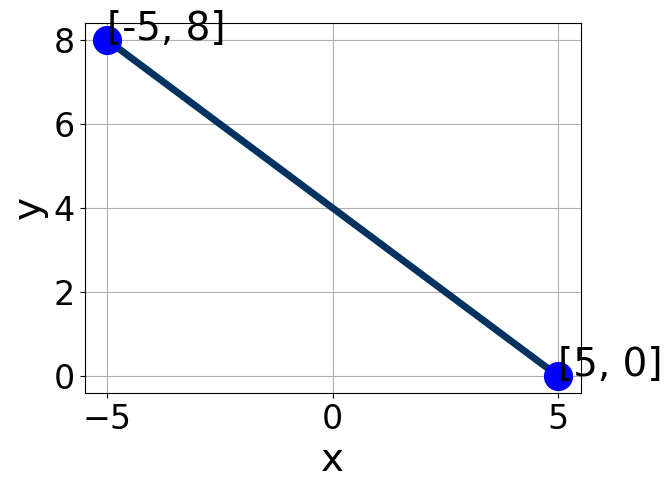
\includegraphics[width=0.5\textwidth]{../Figures/linearGraphToStandardCopyA.png}
\end{center}
\begin{enumerate}[label=\Alph*.]
\item \( A \in [-0.9, 1.8], \hspace{3mm} B \in [-1.3, -0.7], \text{ and } \hspace{3mm} C \in [-5, -2] \)
\item \( A \in [-4.3, -2.6], \hspace{3mm} B \in [-5.3, -4.9], \text{ and } \hspace{3mm} C \in [-22, -15] \)
\item \( A \in [-0.9, 1.8], \hspace{3mm} B \in [-0.5, 1.5], \text{ and } \hspace{3mm} C \in [3, 12] \)
\item \( A \in [2.2, 5.6], \hspace{3mm} B \in [1.5, 7.3], \text{ and } \hspace{3mm} C \in [16, 23] \)
\item \( A \in [2.2, 5.6], \hspace{3mm} B \in [-5.3, -4.9], \text{ and } \hspace{3mm} C \in [-22, -15] \)

\end{enumerate} }
\litem{
Solve the equation below. Then, choose the interval that contains the solution.\[ -2(18x -11) = -15(-17x + 16) \]\begin{enumerate}[label=\Alph*.]
\item \( x \in [0.86, 0.95] \)
\item \( x \in [0.7, 0.88] \)
\item \( x \in [0.99, 1.04] \)
\item \( x \in [-0.91, -0.7] \)
\item \( \text{There are no real solutions.} \)

\end{enumerate} }
\litem{
Solve the equation below. Then, choose the interval that contains the solution.\[ -17(-16x -15) = -11(-19x -10) \]\begin{enumerate}[label=\Alph*.]
\item \( x \in [-4.1, -1.3] \)
\item \( x \in [4.2, 6.5] \)
\item \( x \in [-6.1, -5.2] \)
\item \( x \in [-1.1, 0.4] \)
\item \( \text{There are no real solutions.} \)

\end{enumerate} }
\litem{
First, find the equation of the line containing the two points below. Then, write the equation as $ y=mx+b $ and choose the intervals that contain $m$ and $b$.\[ (-5, 2) \text{ and } (-4, 11) \]\begin{enumerate}[label=\Alph*.]
\item \( m \in [5, 15] \hspace*{3mm} b \in [47, 59] \)
\item \( m \in [5, 15] \hspace*{3mm} b \in [-48, -45] \)
\item \( m \in [-11, -5] \hspace*{3mm} b \in [-28, -21] \)
\item \( m \in [5, 15] \hspace*{3mm} b \in [4, 14] \)
\item \( m \in [5, 15] \hspace*{3mm} b \in [11, 21] \)

\end{enumerate} }
\litem{
First, find the equation of the line containing the two points below. Then, write the equation as $ y=mx+b $ and choose the intervals that contain $m$ and $b$.\[ (-5, -2) \text{ and } (-7, -3) \]\begin{enumerate}[label=\Alph*.]
\item \( m \in [-0.4, 1.8] \hspace*{3mm} b \in [0.39, 1.51] \)
\item \( m \in [-0.4, 1.8] \hspace*{3mm} b \in [3.57, 4.53] \)
\item \( m \in [-2, 0.2] \hspace*{3mm} b \in [-7.28, -5.85] \)
\item \( m \in [-0.4, 1.8] \hspace*{3mm} b \in [2.16, 3.1] \)
\item \( m \in [-0.4, 1.8] \hspace*{3mm} b \in [-1.56, -0.05] \)

\end{enumerate} }
\litem{
Write the equation of the line in the graph below in Standard form $Ax+By=C$. Then, choose the intervals that contain $A, B, \text{ and } C$.
\begin{center}
    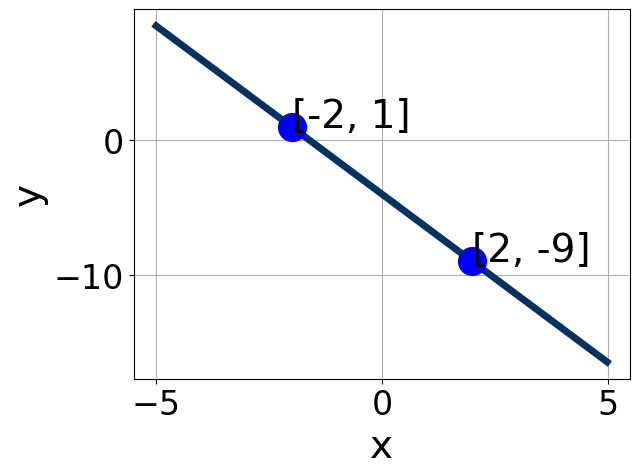
\includegraphics[width=0.5\textwidth]{../Figures/linearGraphToStandardA.png}
\end{center}
\begin{enumerate}[label=\Alph*.]
\item \( A \in [1.7, 4], \hspace{3mm} B \in [-0.17, 1.98], \text{ and } \hspace{3mm} C \in [-6, 1] \)
\item \( A \in [-8.8, -4.3], \hspace{3mm} B \in [-2.22, -1.79], \text{ and } \hspace{3mm} C \in [7, 16] \)
\item \( A \in [3.7, 7.4], \hspace{3mm} B \in [1.44, 2.49], \text{ and } \hspace{3mm} C \in [-11, -7] \)
\item \( A \in [1.7, 4], \hspace{3mm} B \in [-1.4, -0.3], \text{ and } \hspace{3mm} C \in [4, 7] \)
\item \( A \in [3.7, 7.4], \hspace{3mm} B \in [-2.22, -1.79], \text{ and } \hspace{3mm} C \in [7, 16] \)

\end{enumerate} }
\end{enumerate}

\end{document}